\chapter{Boundary Conditions}

see exercise 3.2

\section{Location}
The Romano Port is located at the west-coast of Albania in the Adriatic Sea, 7.5 km north from the city Durr\"{o}es and around 30 km from the capital of Albania Tirana. 
Albania has a HDI (Human Development Index) of 7.33 which puts the country to the "high human development category" according to the HDI report of the UN 2015 like Algeria, Brazil or Turkey. For construction this is a medium-good working conditions it is recommended to use local available equipment and local workers.

\section{Subsoil}
Subsoil matters are not included in this breakwater design. It is assumed, that the soil can resist all loads and that no soil-improvement needs to be done.

\section{Bathymetry}
Bathymetry data were generated using navionics\footnote{webapp.navionics.com}. The bathymetry from this website was copied in CAD where several bathymetry shots could be combined with each other to get a more detailed bathymetry in the necessary parts. Due to the needed xy-data a line with the exact depth values can be exported from CAD and imported into SwanOne.

\section{Additional Water Level}
Due to the following factors the water level rises for the design conditions with 1.3 m according to the mean water level:
\begin{itemize}
\item Tidal differenz: +0.211
\item Sea Level Rise: $0.005 m/year * 100 years = +0.5 m$
\item Seasonal effects: +0.07
\item Atmospheric pressure drop: +0.33 m
\item Wind set-up + seiches: +0.17	
\end{itemize}
Which leads to an increase of the water level in a hundred years for the combination of all effects of 1.281 m which will be considered as 1.3 m to get some small extra safety as an engineering approach.
\section{Waves}
Wave heights and the return period of wave events are essential for determine the dimensions of a breakwater. Especially for estimating the size of the amour layer and hence the size of under-layer material, is the wave hight the dominant parameter. Furthermore the order of the run-up and over-topping magnitude is mainly dependent on the wave hight.
\subsection{Design storm}
The design storm with less than 20\% probability of failure of the breakwater within a lifetime of 100 years returns every 500 years.
The available 22 years of (modelled) wave data\footnote{ARGOSS XX} close to the site is analysed in a Peak over Threshold analysis using a threshold of $H_s=1.5m$, a storm duration of nine hours and a Weibull distribution to extrapolate the data. The wave-data from Argoss were checked for reliability (see appendix).
This yields a significant wave height of $H_{ss}=7.91m$ for a 500 year storm, which is chosen to be the deep water design wave height: $H_{ss,d}=7.91m$.

According to the distribution of the wave hight over peak wave periods from the wave model of Argoss %(appendix \ref{Distribution_pperiod}) 
the peak period was chosen to be 11 seconds.
The Distribution of the wind and the wind speed at 10 m hight was created through the Argoss data set too and shows velocities up to 20 m/s with varying directions
%\ref{Windrose}
. The main  directions are NW, N, NE, SSE and S but for the model just NW and S winds are considered with 20 m/s because of the influence at the breakwater as a worst case scenario.

\subsection{Near-shore Wave model}
SwanOne was used to estimate the wave development at near-shore. The Input parameters are in this case:
\begin{itemize}
\item The generated two dimensional bathymetry
\item The additional water level
\item The wave hight
\item Peak period
\item Wind velocity
\item Angle of incidence 	
\end{itemize}

\begin{figure}[H]
\center
\fbox{
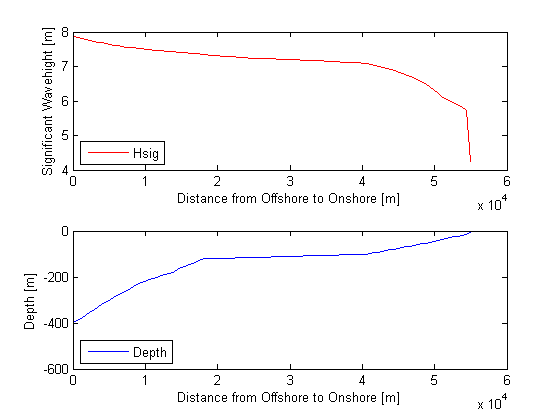
\includegraphics[width=\textwidth]{images/Hsig_Depth_Plot.png} 
}
\caption{Significant Wave Hight and Depth Plot}
\label{Hsig_Depth_Plot}
\end{figure}
In the Swan model additional wind was  included but the set-up due to wave action was neglected, because it is included in the offshore wave data we gained and currents were neglected due to the location in the Mediterranean See with hardly any currents.
Bathymetry,additional water level, wave hight, wind velocity and peak period were determined before, but now different angles of wave attack need to be considered.
For determine which angles are of interest for the occurrence of sea and swell waves the Argoss data are checked again 
%\ref{wavedata_angle}
. As a result from the analysis the dominant direction for waves to occur are NW and S, which matches with the geographical expectations. Due to the orientation of the breakwater at the coast the waves from NW will arrive with a very large angle close to 90$^\circ$ according to the breakwater why the wave energy attacking the breakwater is quite small. Because of the small fetch length just wave with relative low energy will arrive perpendicular to the breakwater. The biggest influence is expected to come from the south and thus the angle of the waves to attack the breakwater will be around 45$^\circ$ which is the value used for the modulation in SwanOne. 
The model was simulating with a grid size of around 5.55 m per cell and 10,000 time steps per simulation to get an accurate result.
The final Simulation is shown in figure \ref{Hsig_Depth_Plot} and the actual value for the significant design wave hight from a one in 500 years storm at the near-shore in a depth of 12 meter is 5.614 m.
\section{Reference levels}
As shown in table \ref{tab:tidal_level} the relative Albanian Level (AL) ,which is +0.535 m above Mean Sea Level, leads to the rewriting of tidal elevations. Every water level in this assignment will be given according to AL.
\begin{center}
\begin{table}[!htb]
\begin{tabu}{X[2l] X[2c]}
\toprule[2pt]
\textbf{Tide} & \textbf{Water Level [m AL]} \\
\\
\midrule
HAT & -0.324\\
\\
HHWS & -0.336\\
\\
MHWS & -0.349\\
\\
MHW & -0.421 \\
\\
MHWN & -0.476\\
\\
MLWN & -0.605\\
\\
MLW & -0.652\\
\\
MLWS & -0.7\\
\\
LLWS & -0.71\\
\\
LAT & -0.722\\

\bottomrule[2pt]
\end{tabu}
\caption{Tidal water levels at Durr\"{o}es}
\label{tab:tidal_level}
\end{table}
\end{center}


\section{Summary}
\begin{center}
\begin{table}[!htb]
\begin{tabu}{X[2l] X[2c]}
\toprule[2pt]
\textbf{Boundary} & \textbf{Value} \\
\\
\midrule
Location & medium-good conditions\\
\\
Subsoil & Not of Concern\\
\\
Reference Level & +0.535 m MSL\\
\\
Bathymetry & see figure \ref{Hsig_Depth_Plot} \\
\\
Additional wwater level & +1.3 m\\
\\
Design storm & $H_{design}=7.912 m$ $T_{design}=11 s$ \\
\\
Significant wave hight & 5.614 m\\
\bottomrule[2pt]
\end{tabu}
\caption{Summary of all boundary conditions at Porto Romano}
\label{tab:summary_boundary}
\end{table}
\end{center}
 